
\subsection{Алгоритмы для подготовка задания}
% \label{part:alghoritm_intro}

\subsubsection{Получение исходных данных о береговой линии}

В разделе~\ref{sec:task_intro} были сформулированы основные требования к блоку формирования и подготовки задания.
Вся логика выполнения метода базируется на описанных в нем (на стр.~\pageref{text:line_prop}) требованиям к береговой линии.

Исходными данными к началу расчета является \texttt{GeoJSON} файл с сохраненным в нем береговой линией (рисунок~\ref{pic:NVRSK_обзор_OSM_clear}).

\begin{figure}
    \begin{center}
	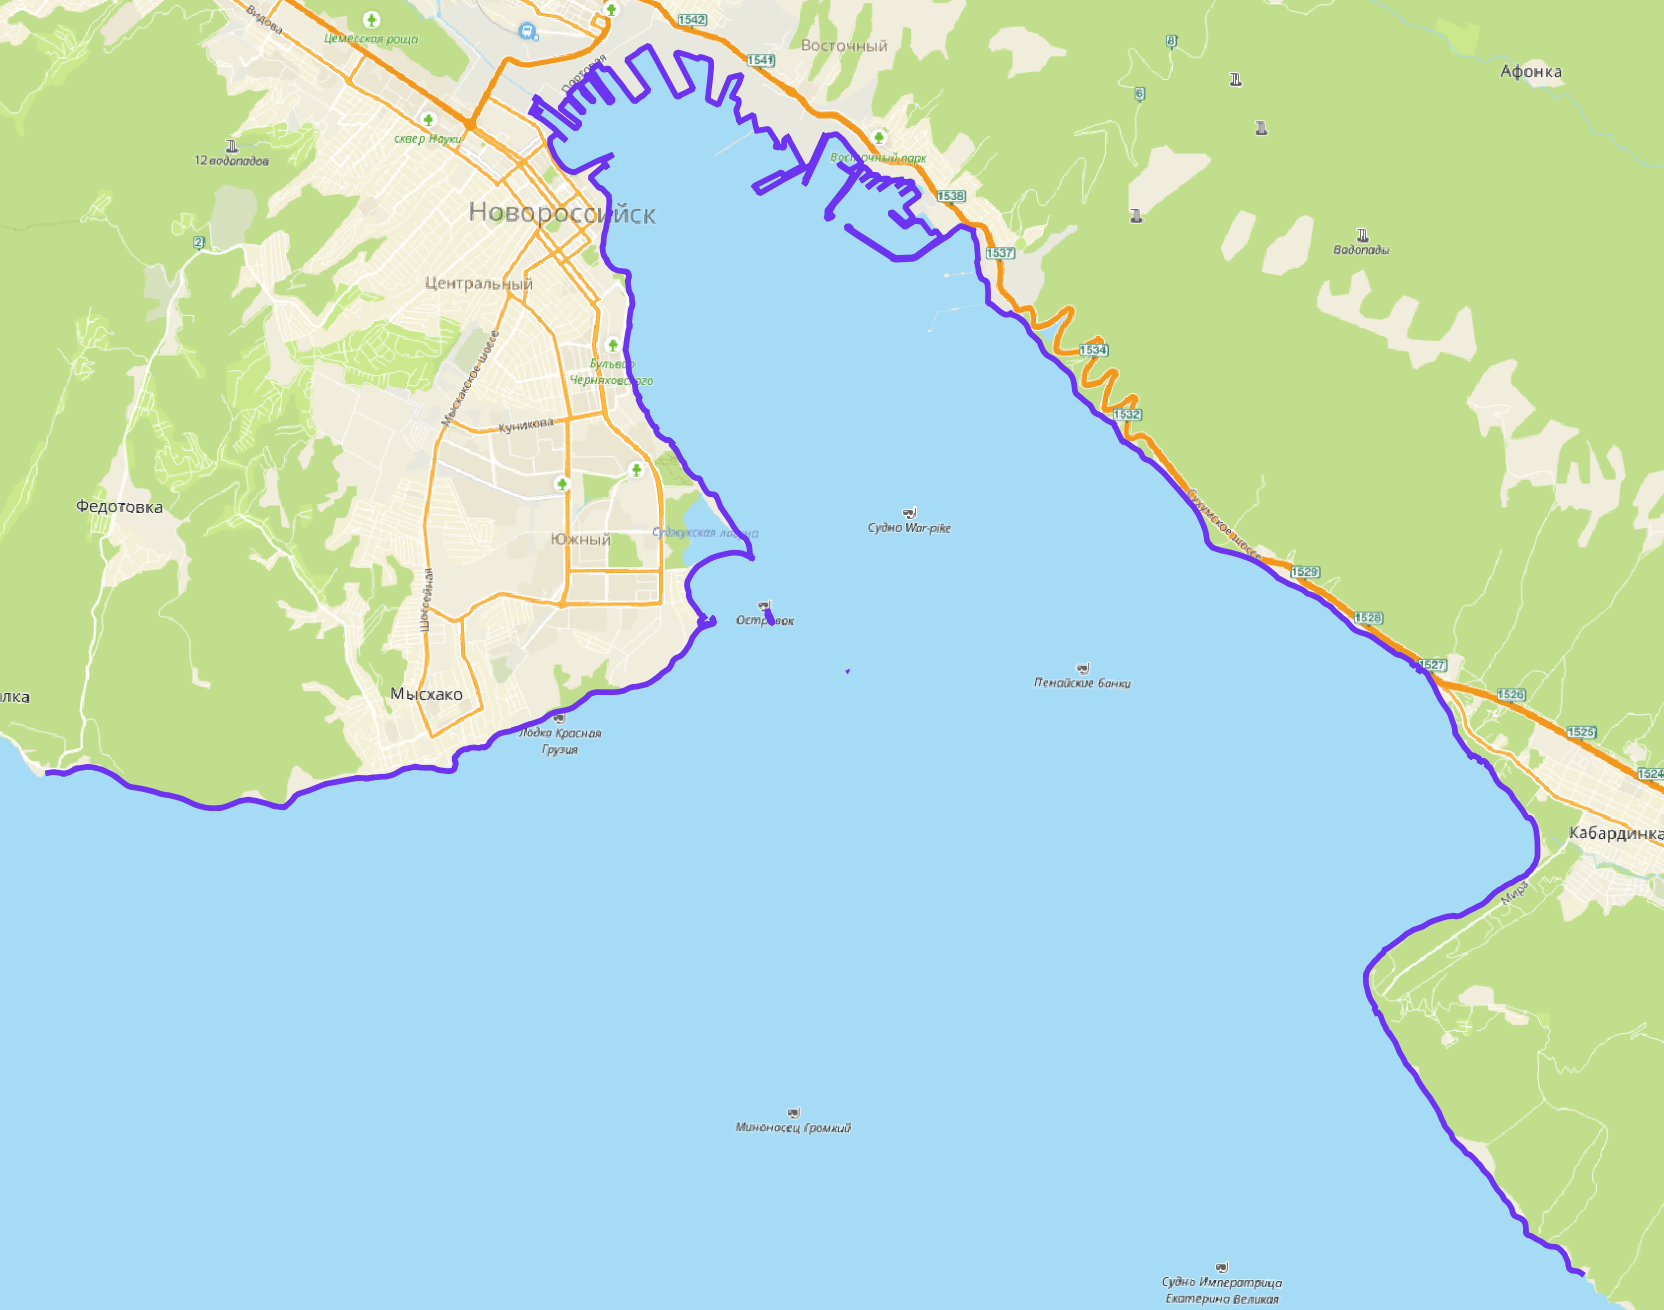
\includegraphics[width=100mm]{fig/part_2/alghoritm/NVRSK_обзор_OSM_clear.png}
	\caption{-- Рассматриваемая в примере часть береговой динии}
	\label{pic:NVRSK_обзор_OSM_clear}
    \end{center}
\end{figure}

При этом поддерживается любой тип записи линий (\texttt{LineString} (одна линия) и \texttt{MultiLineStringring} (набор линий)).

Для удобства пользователя в программе реализованы инструменты автоматического получения этих объектов внутри заданных по координатам границ из следующих доступных данных:
\begin{itemize}
    \item загрузка с серверов OSM напрямую через \texttt{osmx};
    \item выделение данных их pbf файлов GeoFabrik;
    \item выделение подмножества данных из векторных файлов (\texttt{shapefiles}, \texttt{GeoJSON}) содержащих информацию о глобальном положении берегов (например данных S2Coast-2023\cite{Duan2026S2Coast2023} рассмотренных на стр.~\pageref{sec:open_coastline_data}).
\end{itemize}

Следует отметить, что на данном этапе формируется лишь \enquote{опорный} слой береговых линий к которому по сути предъявляется единственное требование -- содержать в себе только линейные объекты, относящиеся к береговой линии.

Уже на этом этапе появляется первая проблема -- в текущее время многие сервера OSM ограниченно доступны с территории РФ.
Таким образом, выделение подмножества их локальных файлов представляется наиболее стабильным.
Следует отметить, что выделения объектов GeoFabrik в программе выполняется через свободно распространяемую утилиту \texttt{osmium}, необходимые команды которой прокидываются через python обертку.

Рассмотрев фрагменты береговых линий (рисунок~\ref{pic:NVRSK_OSM_S2C}), полученных их OSM (\enquote{А}) и S2Coast-2023 (\enquote{Б}) можно визуально найти первую их проблем -- не все реально существующие объекты присутствуют в них.
В случае S2Coast-2023 низкое пространственное разрешение (10 м) не позволяет надежно зафиксировать положение меньших в сечении объектов, из-за чего можно наблюдать пропуски в линиях, определяющих положение узких молов и нефтеналивных терминалов.
Дополнительно следует отметить большее присутствие шумов береговой линии из S2Coast-2023, вызванное векторизацией растровых спутниковых снимков.

\begin{figure}
    \begin{center}
	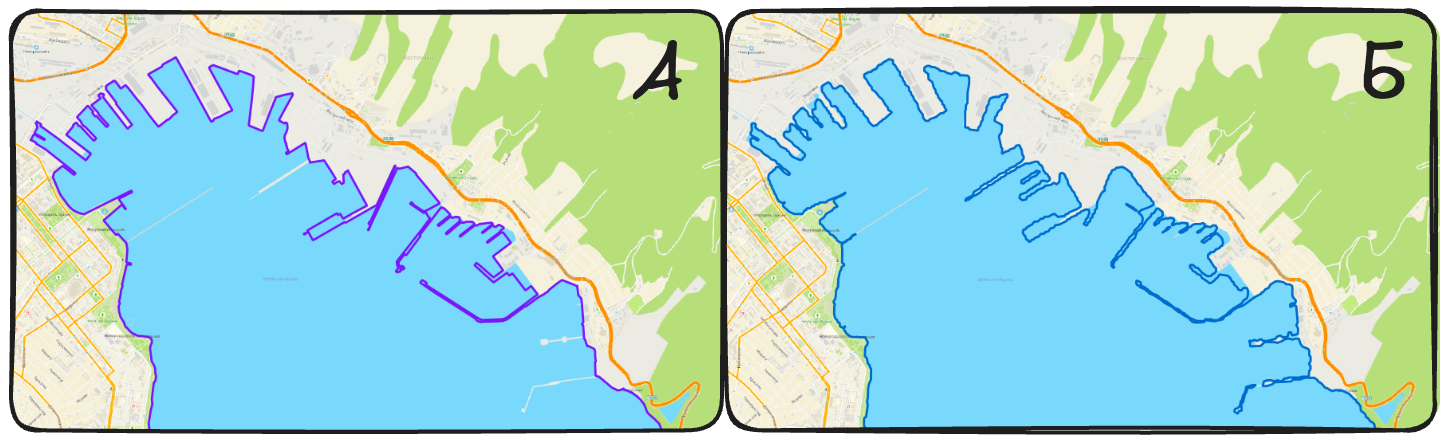
\includegraphics[width=\textwidth]{fig/part_2/alghoritm/NVRSK_OSM_S2C.png}
	\caption{-- Сравнение береговой линии OSM (\enquote{А}) и S2Coast-2023 (\enquote{Б})}
	\label{pic:NVRSK_OSM_S2C}
    \end{center}
\end{figure}

Исходя из этого, при анализе берега в границах городских территорий, описываемого совокупностью прямых отрезков, перспективнее опираться на OSM данные.
Визуальный анализ территорий, содержащих положение естественной береговой линии, показывает равное качество векторизации в обоих наборах данных.

Наряду с пропусками данных в наборах в них скрыта еще одна потенциальная труднотсь -- они все сегменированы внутри себя.
Так S2Coast-2023 разделен на тайлы в 1 градус по широте и долготе, а OSM весь состоит из довольно хаотической последовательности линий проведенных в разное время, разными людьми и в разных направлениях.
Добавим к этому то, что все эти сегменты часто не замкнуты со своими соседями мы получаем внешне привлекательную, но потенциально проблемную к последующей обработке сущность.

Не решив вопросы связности  и сонаправленности линий, мы многократно усложним как алгоритмы выделения точек на линии, так и расчеты векторов нормали с единым, согласованным, направлением к морю.
Вспомнив также ранее упомянутое обстоятельство с пропуском реальных объектов, реализуем отдельный алгоритм подготовки векторных данных с выделением единой результирующей береговой линии.

Приняв рассогласованность и множественность линейных объектов в наборе не как трудность, а как данность, мы сразу получаем естественную возможность к добавлению пропущенных в них объектов.
Так на рисунке~\ref{pic:NVRSK_line_bulding} (\enquote{А}) красными линиями выделены вручную отвекторизованные молы и причалы.
Отдельно отметим, что узлы добавленных линий не совпадают ни с узлами, ни с линиями существующей в наборе береговой линии.

Дополнительно отметим также тот факт, что аналогично случаю восстановления существующих объектов на этом этапе могут быть добавлены объекты подлежащие предпроектному анализу.
В результате чего становится возможным выполнить оценку влияния перспективных к строительству объектов в контексте существующих объектов прибрежной инфраструктуры.

\subsubsection{Выделение главной береговой линии}
\label{sec:main_line_bulding}

Какой линейный объект мы хотим получить в итоге?
Во-первых, нам нужно отделить главный берег от сопутствующих объектов (мелких островов, повторов в береговых линиях и артефактов от геометрических построений на берегу).
Во-вторых, этот объект должен быть единственным, с четко определенным направлением прохода вершин.
Но как это реализовать?

Изначально положение вершин линий задано в географической системе координат и определено в градусной мере по широте и долготе.
Так как анализ связности сегментов линий предполагает поиск ближайших, соседних, вершин, что требует перепроецирования в прямоугольную систему координат, определяемую по положению центральной точки ограничивающей геометрии (бибокса) данных.

После пересчета этого выполняется \enquote{привязка} (snapping) вершин сегментов друг к другу.
Поиск соседей определяется по заданному пользователю порогу и позволяет исключить случайные, мелкие, разрывы в данных, сократив при этом общее количество линий в наборе.

Дальнейшее объединение сегментов требует определения и анализа точек пересечений сегментов линии между собой.
В результате выделения совместных узлов у пересекающихся объектов формируется набор элементарных сегментов без топологических дыр, позволяющий представить все объекты в виде набора графов.

На следующем этапе производится выделение главной линии графа, которая максимизирует суммарный вес ребер, определяемый пропорционально длине сегментов.
После этого выполняется устранение циклов в графе (петель, возникших из-за ошибок привязки вершин через snapping). 
После выделения главной линии выполняется \enquote{чистка} листьев.
Для ребер графа со степенью узлов 1 считаем длину ветки до ближайшего узла с степенью $≠ 2$, если длина ветки меньше заданного пользователем порога -- она удаляется.
Выполнение этих операций повторяется в несколько итераций до тех пор, пока короткие \enquote{хвосты} не исчезнут.

На очищенном дереве ищем самый длинный путь.
Для чего выбирается произвольная вершина и запускается поиск кратчайших путей с весами по алгоритму Дийкстры.
Выбирая новую вершину, расстояние до которой максимально, выполняем поиск уже относительно нее.
В результате две найденные вершины и будут границами главной береговой линии.

Множество ребер выходящее за пределы главной линии определяется как второстепенное.
После чего формируется два выделенных набора линий сохранящихся в соответствующие им файлы.
Результат выделения второстепенных линий представлены на рисунке~\ref{pic:NVRSK_line_bulding} (\enquote{Б} -- \enquote{Г}).

\begin{figure}
    \begin{center}
	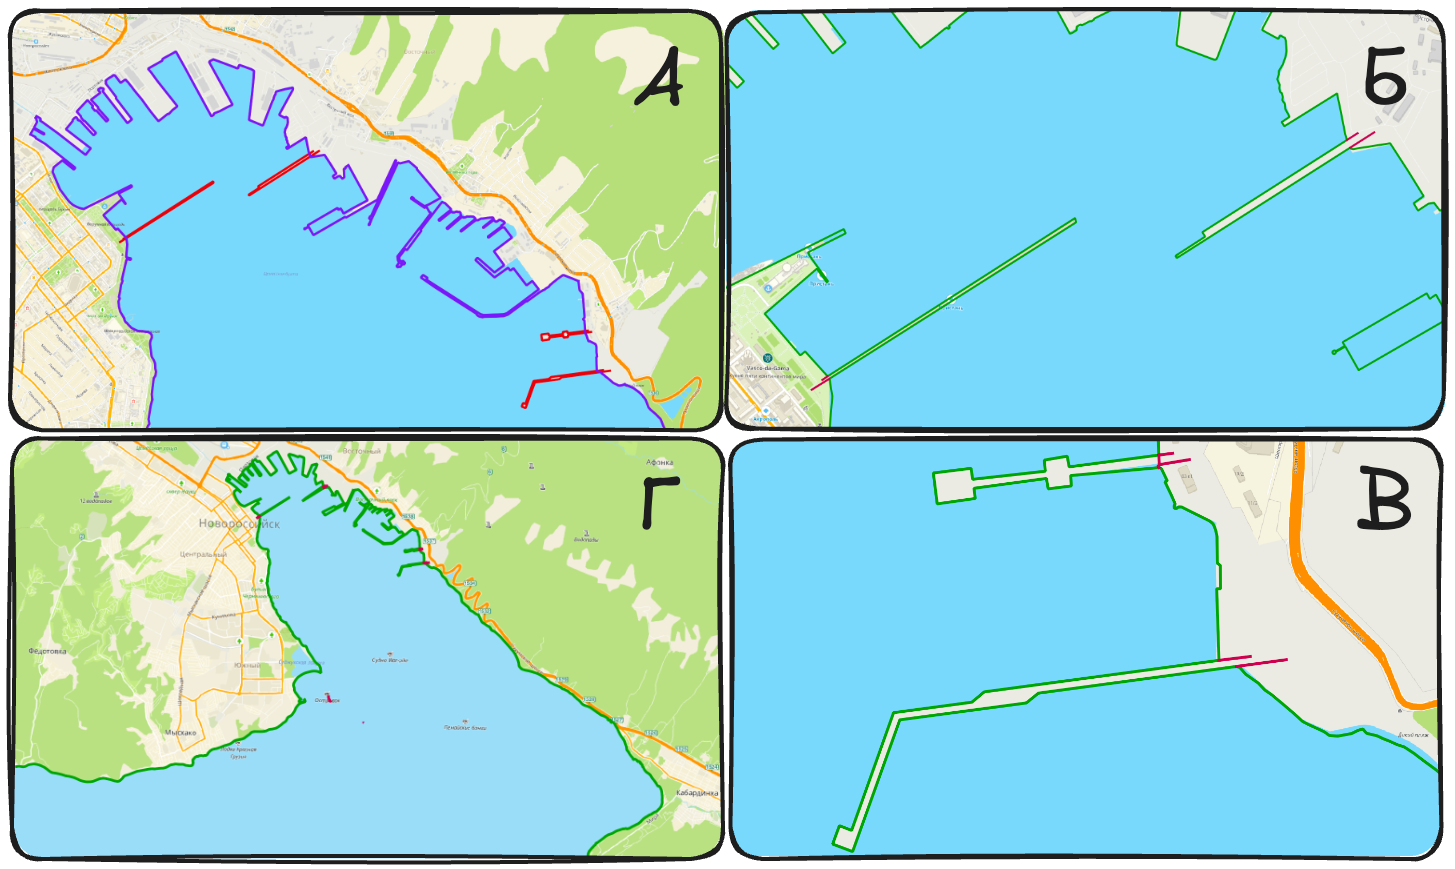
\includegraphics[width=\textwidth]{fig/part_2/alghoritm/NVRSK_line_bulding.png}
	\caption{-- Выделение главной береговой линии}
	\label{pic:NVRSK_line_bulding}
    \end{center}
\end{figure}

\subsubsection{Выделение точек}

Ранее в разделе~\ref{sec:task_intro} было определено, что расчеты будут выполняться для точек, принадлежащих береговой линии.
В реализованной версии программы реализовано 4 основных стратегии продемонстрированные на рисунке~\ref{pic:NVRSK_points_strategys}:
\begin{itemize}
    \item выделение точек, как узлов линии (\enquote{А});
    \item выделение точек с равным шагом по пикетажу линии (\enquote{Б});
    \item выделение точек по \enquote{радиусу} (на равном евклидовом расстоянии от предыдущей) вдоль трассы (\enquote{В});
    \item комбинированная стратегия, объединяющая результаты набора предыдущих в единое множество.
\end{itemize}

\begin{figure}
    \begin{center}
	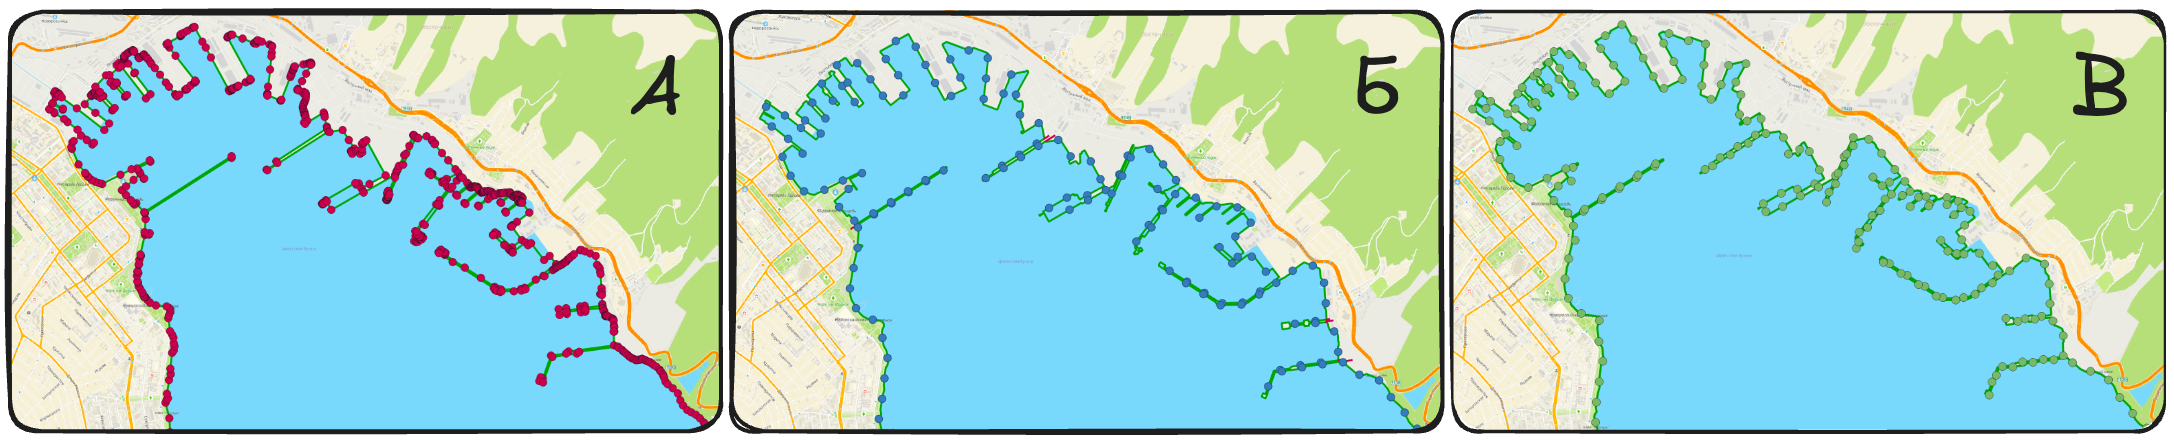
\includegraphics[width=\textwidth]{fig/part_2/alghoritm/NVRSK_points_strategys.png}
	\caption{-- Стратегии выделения точек для расчета}
	\label{pic:NVRSK_points_strategys}
    \end{center}
\end{figure}

Визуально оценивая репрезентативность и объем выделенных наборов точек, можно сделать вывод, что стратегия выделения узловых точек, хотя и кажется изначально наиболее естественной, приводит в общем случае к худшим результатам.
Выделенные таким образом точки распределены в пространстве наименее равномерно и слабо описывают инженерные объекты (рисунок~\ref{pic:NVRSK_bad_nodex_ex}).

\begin{figure}
    \begin{center}
	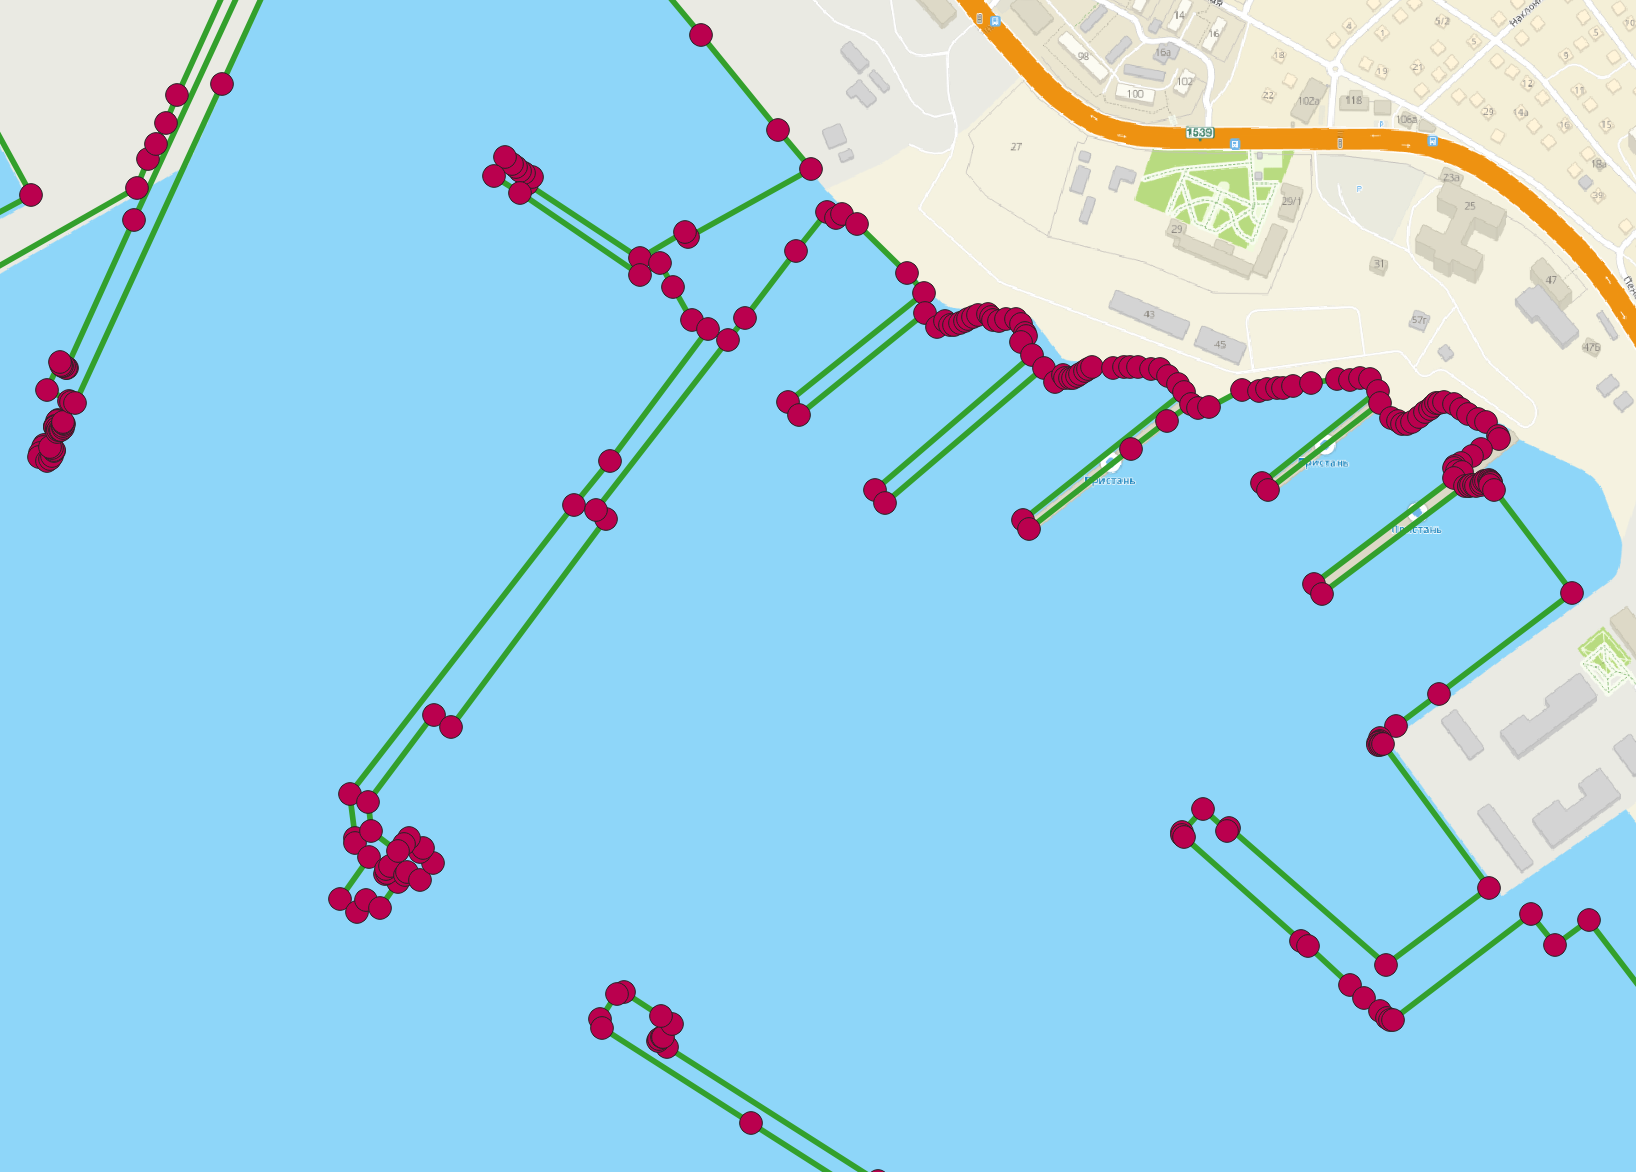
\includegraphics[width=100mm]{fig/part_2/alghoritm/NVRSK_coasteral_poinr_nodes_bad_example.png}
	\caption{-- Пример выделения узловых точек на инженерных объектах}
	\label{pic:NVRSK_bad_nodex_ex}
    \end{center}
\end{figure}

Стратегии выделения точек по равному пикетажу и равному радиусу показывают схожие между собой результаты.
Однако способ с постоянным радиусом позволяет выделять более симметричные точки относительно осей вытянутых узких объектов, что в перспективе может упростить анализ уязвимости берегозашитных гидротехнических сооружений.
В связи с этим, в дальнейших примерах расчетов был выбран набор данных сформированный этим способом.

Хотя в рассматриваемом примере необходимость искуственного добавления точек вручную не рассматривается, в разработанном алгоритме нет технических ограничений на то, чтобы пользователь добавил их в любой удобной для себя программной среде. 

\subsubsection{Вычисление нормалей}

В разделе~\ref{sec:task_intro} (стр.~\pageref{eq:norm_vect_line}) одним из необходимых условий была заявлена необходимость сопоставления каждой анализируемой точке вектора нормали к берегу.
Технически положение вектора нормали будет косвенно определять направление береговой лини в окрестности рассматриваемой точки. 

На первом этапе вычислений выполняется проверка того, что набор точек не пуст и что у него присутствует информация о конкретной системе координат (CRS).
После этого координаты точек пересчитываются в прямоугольную систему координат, в которой находится береговая линия.
Далее для каждой точки определяется ее положение точки на береговой линии.
Очевидно, что для набора точек, сформированного по описанным ранее стратегиям, эти условия выполнятся автоматически, но допуская возможность \enquote{ручного} определения точек пользователем выполняемые проверки и повторные вычисления гарантируют правильность дальнейших расчетов при минимальной \enquote{стоимости} избыточных вычислений.

Далее вокруг рассматриваемой точки задается симметричное окно $[s-\Delta,\, s+\Delta]$, где $\Delta$ -- задаваемый в метрах параметр ширины окна.
Следует отметить, что величина задаваемой $\Delta$ определяет чувствительность положения нормали к локальным изменениям линии.
Так, приняв значение $\Delta$ равным половине расстояния между точками, мы получим \enquote{сглаженное} описание всей береговой линии, в то время когда $\Delta → 0$ мы сможем получить более строгое перпендикулярное направление вектора к касательной берега в рассматриваемой точке.

По этим двум границам окна $[s-\Delta,\, s+\Delta]$ на линии вычисляются точки $p_0$ и $p_1$.

Вектор:
\begin{equation}
    (dx,dy) = (p_1.x-p_0.x,\; p_1.y-p_0.y)
\end{equation}
используется как приближение локальной касательной к береговой линии в окрестности рассматриваемой точки.
После этого касательная нормируется до единичного вектора:
\begin{equation}
    \mathbf{t} = (t_x,t_y) = \frac{(dx,dy)}{\sqrt{dx^2+dy^2}}.
\end{equation}

Единичный нормальный вектор строится как вектор, перпендикулярный касательной.

На этом этапе расчета возникает естественная неоднозначность -- куда повернуть вектор: налево или направо?
От этого выбора будет зависеть будет ли вектор направлен в сторону суши или моря.
Так для левой нормали используется поворот на $90^\circ$, а для правой -- на $-90^\circ$. В коде это реализовано так:
\begin{itemize}
    \item \texttt{left}: $(n_x,n_y)=(-t_y,\; t_x)$;
    \item \texttt{right}: $(n_x,n_y)=(t_y,\; -t_x)$.
\end{itemize}


Ранее (на стр.~\pageref{eq:norm_vect_line}) было определено условие о направлении вектора к морю.
Технически, предполагая наличие батиметрических данных, этот выбор может быть легко алгоритмизирован, но в текущей реализации программы он делегирован пользователю, выбирающему направление вручную. 
С учетом того, что в результате работы алгоритма описанного в~\ref{sec:main_line_bulding} мы получили согласованную по направлению линию сделанный выбор будет одинаково правильным или ошибочным для всего набора точек.

После расчета компоненты вектора нормали, он дополнительно нормируется и переводится в азимут:
\begin{equation}\label{eq:azimuth_calc}
    \alpha = \bigl(\operatorname{degrees}(\operatorname{atan2}(n_x,n_y)) + 360\bigr)\bmod 360.
\end{equation}

На основе рассчитанного значения получается направление нормали в градусах, удобное для последующего анализа и визуализации (рисунок~\ref{pic:NVRSK_port_norm_vectors}).

\begin{figure}
    \begin{center}
	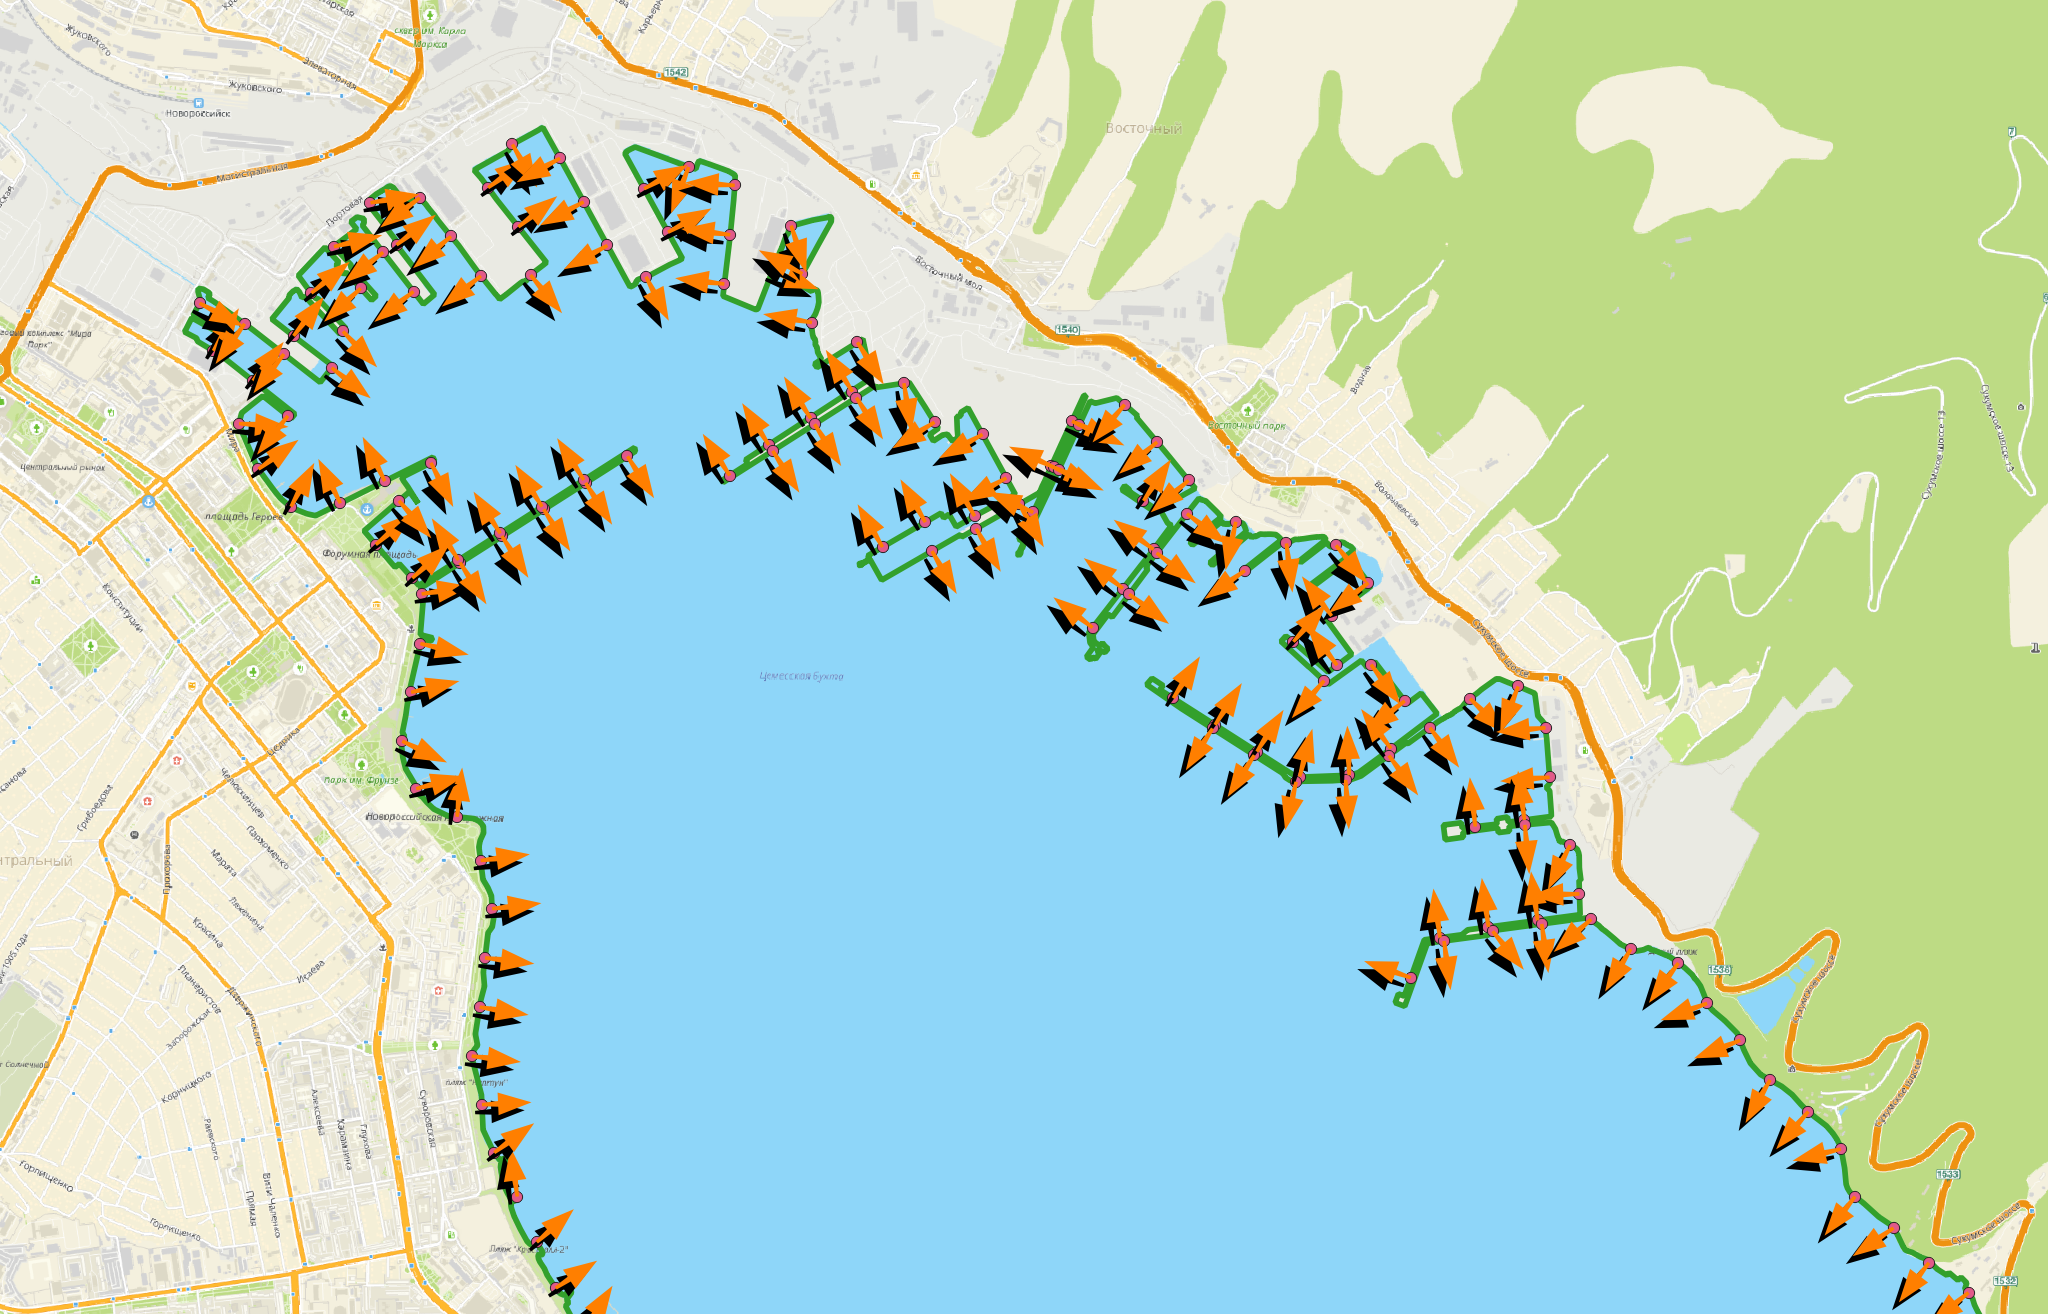
\includegraphics[width=100mm]{fig/part_2/alghoritm/NVRSK_vector_port.png}
	\caption{-- Результаты расчета векторов номали}
	\label{pic:NVRSK_port_norm_vectors}
    \end{center}
\end{figure}
